
The closed loop block diagram for the outer loop of the ball on beam system including an integrator is shown in Figure~\ref{fig:hw_ballbeam_PID_root_locus}.  
\begin{figure}[htbp]
   \centering
   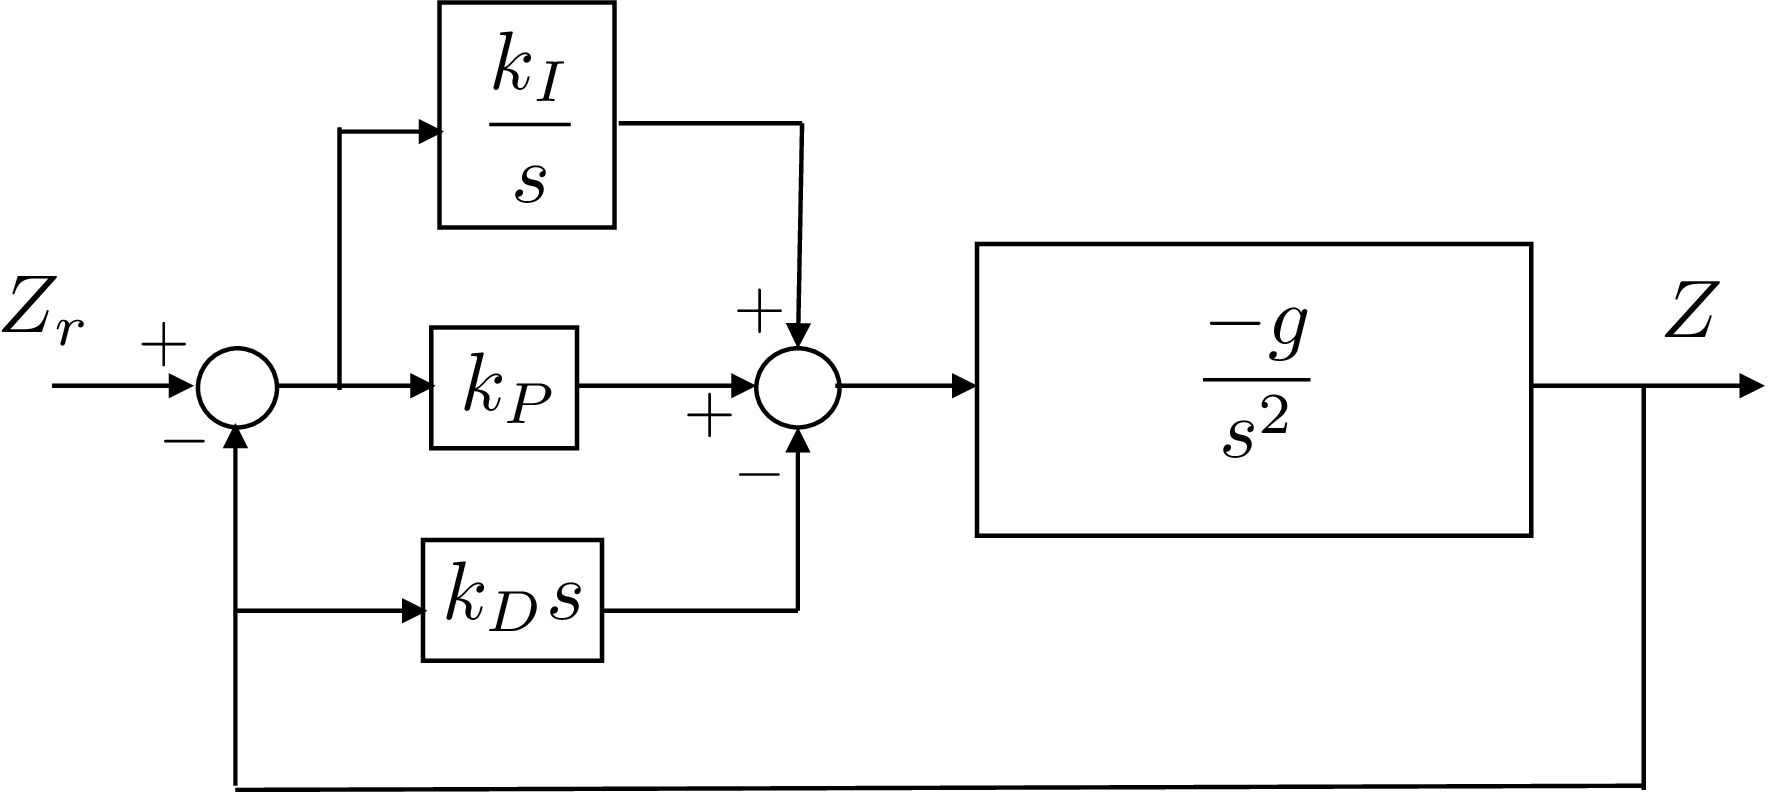
\includegraphics[width=0.6\textwidth]{6_design_studies/figures/hw_ballbeam_PID_root_locus.pdf}
   \caption{PID control for the outer loop of the ball on beam system.}
   \label{fig:hw_ballbeam_PID_root_locus}
\end{figure}
The characteristic equation is given by
\[
1+P(s)C(s) = 1+\left(\frac{-g}{s^2}\right)\left(\frac{k_Ds^2+k_Ps+k_I}{s}\right) = 0.
\]
Rearranging gives
\[
s^3 + (-gk_D)s^2 + (-gk_P)s + (-gk_I) = 0.
\]
Therefore, in Evan's form we have
\[
1 + k_{I}\left(\frac{-g}{s^3 + (-gk_D)s^2 + (-gk_P)s}\right) = 0.
\]
The appropriate Matlab command is therefore
\begin{lstlisting}
>> L = tf([-g], [1, -g*kd, -g*kp, 0]);
>> figure(1), clf, rlocus(L);
\end{lstlisting}
